\documentclass[preprint,authoryear,12pt]{noelsarticle}
%\documentclass[preprint,12pt]{elsarticle}
%\documentclass[final,3p,times,authoryear]{elsarticle}
%\documentclass[final,3p,times]{elsarticle}

\usepackage{tikz}
\usepackage{hyperref}
\usepackage{verbatim}
\usepackage{comment}
\usepackage{boxedminipage}
\usepackage{amssymb}
\usepackage{listings,lsthaskell,lstprolog,lstegl,lstesl,lstfsml,lstjava,lstdot}

\newcommand{\m}[1]{\ensuremath{\mathit{#1}}}
\newcommand{\slepro}{\textsc{SlePro}}
\newcommand{\concept}[1]{\emph{#1}}
\definecolor{codebackground}{rgb}{0.97,0.97,0.97}
\definecolor{gray}{rgb}{0.5,0.5,0.5}
\definecolor{keyword}{rgb}{0.5,0.0,0.5}
\definecolor{comment}{rgb}{0.3,0.5,0.3}
\definecolor{code}{rgb}{0.0,0.0,0.3}
\definecolor{ncode}{rgb}{0.0,0.3,0.3}
\definecolor{scode}{rgb}{0.3,0.0,0.3}
\definecolor{static}{rgb}{0.0,0.0,0.3}
\newcommand{\ncode}[1]{\texttt{\textup{\color{ncode}#1}}}
\newcommand{\jcode}[1]{\texttt{\textup{\color{code}#1}}}
\newcommand{\scode}[1]{\texttt{\textup{\color{scode}#1}}}
\newcommand{\static}[1]{\texttt{\textsl{\color{static}#1}}}

\newcommand{\codefigure}[3]{
\begin{figure}[t!]
\begin{boxedminipage}{\hsize}
\mbox{}\hfill{}{\small\textit{\href{http://github.com/slebok/slepro/tree/master/#2}{#2}}}
\lstinputlisting[language=#3]{../../#2}
\end{boxedminipage}
\caption{#1.}
\label{#2}
\medskip
\end{figure}}

\lstset{%
  fontadjust=true,%
  showstringspaces=false,%
  basicstyle=\small\sffamily,%
  keywordstyle=\color{keyword},%
  commentstyle=\color{comment}\rmfamily\itshape\small,%
  columns=fullflexible,%
  tabsize=2,
%  numbers=left,                   % where to put the line-numbers
  numberstyle=\tiny\color{gray},  % the style that is used for the line-numbers
  backgroundcolor=\color{codebackground},
  stepnumber=2,                   % the step between two line-numbers
%  numbersep=5pt,                  % how far the line-numbers are from the code
 % aboveskip=1.5\medskipamount,%
 % belowskip=1.5\medskipamount,
aboveskip = 0pt,
belowskip = 0pt,
  %breaklines=true
}

\newcommand{\wikipediafn}[2]{\footnote{\url{#1}---last visited #2.}}
\newcommand{\ooo}[1]{\textsf{101#1}}

%% \biboptions{comma,round}
% \biboptions{}

\begin{document}

\begin{frontmatter}

\title{Another DSL primer}

\author{Ralf L\"ammel}

\address{Software Languages Team\\University of Koblenz-Landau, Germany}

\begin{abstract}
  We model a domain-specific language FSML for Finite State Machines
  (FSMs). The language model encompasses concrete a textual syntax, a
  term-based abstract syntax, a graph-based visual syntax, extra
  constraints for well-formedness, a simulation semantics, and a
  code-generation semantics for representing and executing FSMs in
  Java. The key motivation for the present model of FSML to be
  explainable exhaustively in terms of simple formalisms and idioms,
  all layered on top of Prolog. The FSML development is part of the
  \slepro{} project; see \url{https://github.com/slebok/slepro}.

\bigskip

\noindent
\textbf{Acknowledgement}: {\small This document and the underlying
  development are parts of a broader effort on language modeling and
  software language engineering---joint work with \emph{Anya Helene
    Bagge}, University of Bergen. Helpful interaction with and
  feedback by Andrei Varanovich, University of Koblenz-Landau, is also
  gratefully acknowledged.}

\medskip

\noindent
\textbf{Version}

0.00002 as of 25 November 2013.

\medskip

\noindent
\textbf{Repository location of document}: 

\url{https://github.com/slebok/slepro/tree/master/docs/fsml}.
\end{abstract}

\end{frontmatter}

\pagebreak

%%%%%%%%%%%%%%%%%%%%%%%%%%%%%%%%%%%%%%%%%%%%%%%%%%

\tableofcontents

\pagebreak

%%%%%%%%%%%%%%%%%%%%%%%%%%%%%%%%%%%%%%%%%%%%%%%%%%

\section{Introducing FSML}

%%%%%%%%%%%%%%%%%%%%%%%%%%%%%%%%%%%%%%%%%%%%%%%%%%

\begin{figure}[t!]
\vspace{-77\in}
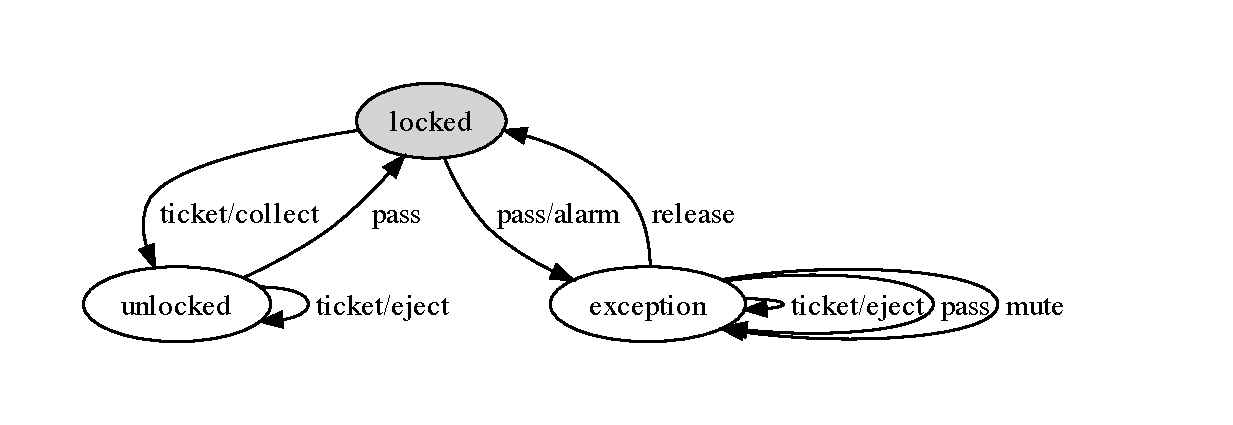
\includegraphics[width=\textwidth]{../../languages/fsml/sample.pdf}
\vspace{-150\in}
\caption{A finite state machine for turnstiles.}
\label{F:turnstile}
\end{figure}

%%%%%%%%%%%%%%%%%%%%%%%%%%%%%%%%%%%%%%%%%%%%%%%%%%

Consider the visual representation of a finite state machine (FSM) for
a turnstile (as used in subway systems). The idea is, of course, that
the customer is supposed to insert a ticket before passing the
turnstile. Thus, the FSM assumes the initial state `locked'. (The
initial state is highlighted by using a filled ellipse.) The input
`ticket' (meaning the insertion of a ticket) causes a transition to
the state `unlocked' and the action `collect'. In this new state, the
input `pass' (meaning the attempt to pass the turnstile) causes a
transition back to the state `locked'. If the input `pass' was made in
the state `locked', then this causes a transition to the state
`exception' and an action `alarm'. The state `exception' rejects the
input `ticket'. The input `pass' does, of course, keeps one in the
state `exception'. The `alarm' can be muted with the input `mute'. We
return to the normal `locked' state upon the input `release'.

We will model a language FSML (FSM language) for modeling
FSMs. Specifically, we will model several aspects of FSML:

\begin{itemize}
\item The visual syntax as used in the figure; see \S\ref{S:visual}.
\item A textual syntax as an alternative concrete syntax; see \S\ref{S:textual}.
\item An abstract syntax useful for representation in programs; see \S\ref{S:abstract}.
\item Extra well-formedness constraints on the abstract syntax; see \S\ref{S:ok}.
\item A reference semantics for the simulation of FSMs; see \S\ref{S:semantics}.
\item A code generator translating FSMs into OO programs; see \S\ref{S:generator}.
\end{itemize}

This primer is concluded by some `food for thought' in
\S\ref{S:concl}. That is, we critically discuss the language model at
hand as well as the underlying approach, thereby also motivating
reproductions of the model as well as variations on the model,
possibly leveraging diverse technologies and techniques.

The FSML development is part of the \slepro{} project. All software
artifacts of this document and all support infrastructure is available
through the repository of the project:

\begin{center}
\url{https://github.com/slebok/slepro}
\end{center}

%%%%%%%%%%%%%%%%%%%%%%%%%%%%%%%%%%%%%%%%%%%%%%%%%%

\section{The concrete textual syntax of FSML}
\label{S:textual}

\codefigure{%
The FSM of \autoref{F:turnstile} in concrete textual syntax}{%
languages/fsml/sample.fsml}{%
fsml}

A textual syntax may break down an FSM into `state declarations',
i.e., states with the associated transitions. Each transition
identifies the relevant input, the optional action, and the target
state. In fact, if the target state is omitted, then this is taken to
mean that the transition's target is the current state. See
\autoref{languages/fsml/sample.fsml} for an illustration.

\codefigure{%
Context-free grammar for the concrete syntax of FSML}{%
languages/fsml/cs.egl}{%
egl}

Let us define the syntax in terms of a context-free grammar. We use an
EGL grammar, where EGL stands for `extended grammar language' and can
be regarded as a variation on the Extended Backus Naur Form. EGL is an
ad-hoc grammar notation that is provided by the \slepro{} project; see
\ref{A:egl} for a self-description. In particular, EGL grammars can
be executed for the purpose of parsing, but we omit all such details
here. See \autoref{languages/fsml/cs.egl} for the grammar. It can be
assumed that the concrete textual syntax, as illustrated in
\autoref{languages/fsml/sample.fsml}, can be parsed indeed
with the present grammar.

%%%%%%%%%%%%%%%%%%%%%%%%%%%%%%%%%%%%%%%%%%%%%%%%%%

\section{The abstract syntax of FSML}
\label{S:abstract}

Eventually, we want to manipulate FSMs in (Prolog) programs. To this
end, we need a suitable abstract syntax. As an aside, there exist
metaprogramming systems that can leverage the concrete syntax
directly, without any need for a separate abstract syntax, but we will
adopt the simpler approach here to indeed use an abstract syntax. In
fact, we assume that abstract syntax trees are (Prolog) terms as in
the sense of term algebras or algebraic specifications.

\codefigure{%
The FSM of \autoref{F:turnstile} in abstract syntax}{%
languages/fsml/sample.term}{%
prolog}

See \autoref{languages/fsml/sample.term} for an
illustration. The abstract syntax describes a FSM as a list of state
declarations, which are in turn tuples (triplets) of the form (\m{V},
\m{Id}, \m{Ts}) where \m{V} is a Boolean saying whether the state is
initial, \m{Id} is the assigned id (name) of the state, and \m{Ts} is
a list of transitions. Each transition is a triplet of the form
(\m{In}, \m{A}, \m{To}) where \m{In} is the input for the transition,
\m{A} is the optional action and \m{To} is the target state. The
optionality of the action is represented such that the missing action
is represented by `[]' and the present action, e.g., `eject', is
represented by `[eject]'.

\codefigure{%
Signature for the abstract syntax of FSML}{%
languages/fsml/as.esl}{%
esl}

Let us define the abstract syntax in terms of a signature that defines
all valid FSM terms. We use an ESL signature, where ESL stands for
`extended signature language' and can be regarded as (quite) a
variation on notations familiar from algebraic specification or (less)
a variation on type systems used in logic or functional
programming. ESL is an ad-hoc signature notation that is provided by
the \slepro{} project; see \ref{A:esl} for a syntax definition of
the signature notation. In particular, ESL grammars can be executed
for conformance checking to see whether a given term conforms to a
given signature, but we omit all such details here. See
\autoref{languages/fsml/as.esl} for the signature. The term in
\autoref{languages/fsml/sample.term} conforms indeed to
the present signature.

\codefigure{%
Concrete to abstract syntax mapping for FSML}{%
languages/fsml/cs-to-as.pro}{%
prolog}

As we intend to parse FSMs via the concrete textual syntax and to
manipulate FSMs though via the abstract term-based syntax, we need a
mapping from the former to the latter. Of course, both syntaxes are
very close to each other in terms of the nonterminals or types defined
and in terms of the structural breakdown. However, some fine details
need to be declared explicitly via a mapping so that parse trees
according to the earlier grammar are precisely mapped to terms that
conform to the signature for the abstract syntax. The mapping is
defined by a Prolog predicate \emph{fsmlMapping}; see the Prolog
clauses in \autoref{languages/fsml/cs-to-as.pro}.

The syntax definition approach of the \slepro{} project assumes such
mappings are indeed predicates with three arguments \m{N}, \m{T1},
\m{T2} as follows. \m{N} is the nonterminal (according to the grammar
for the concrete syntax) whose parse trees are to be mapped, i.e.,
rewritten. \m{T1} is the (imploded) parse tree that just
systematically follows the structure of the grammar. \m{T2} is the
term that should be used in place of \m{T1}. The starting point is an
identity mapping; the mapping predicate only overwrites those cases
where the identity mapping is not appropriate. In
\autoref{languages/fsml/cs-to-as.pro}, the first clause replaces the
list-of-chars representation of FSM names by proper atoms (`strings').
The second clause replaces `initial' by `true' (and `noninitial' by
`false'); it also fills in the target state, when it is missing,
thereby taking care of some syntactic sugar, i.e., the permitted
omission of the target state when it equals the source state of a
transition.

%%%%%%%%%%%%%%%%%%%%%%%%%%%%%%%%%%%%%%%%%%%%%%%%%%

\section{Constraints on the abstract syntax}
\label{S:ok}

The concrete and abstract syntaxes so far do not cover some of the
constraints that we would naturally apply to FSMs. For instance, we
did not rule out so far that FSMs have multiple initial states, which
is probably not useful. Context-free grammars and signatures are
notoriously limited in expressiveness to model such constraints,
whereas they are convenient for the basic definition of structure. We
need to add extra constraints on top of (say) the abstract syntax
definition. In some communities, it is common to actually consider
these constraints to form part of the abstract syntax whereas we
follow another common view that such constraints are considered
separately as in well-formedness or well-typedness judgements used in
type systems for programming languages.

\codefigure{%
Overview of constraints imposed on FSML's abstract syntax}{%
languages/fsml/ok.pro}{%
prolog}

See \autoref{languages/fsml/ok.pro} for the Prolog specification
listing the named constraints that we consider here. Each constraint
gives rise to a separate predicate considered below. Here is short
summary. Constraint \emph{fsmSingleInitial} is meant to ensure that
there is only a single state declaration for an initial
state. Constraint \emph{fsmDistinctIds} is meant to ensure that the
state ids of the state declarations are distinct. Constraint
\emph{fsmResolvable} is meant to ensure that all referenced target
states are declared. Constraint \emph{fsmDeterministic} is meant
to ensure that each given input uniquely defines the target state to
be transitioned to, if any. Constraint \emph{fsmReachable} is meant to
ensure that all declared states are reachable from the
initial state. In \autoref{languages/fsml/ok.pro}, all constraint
predicates are surround by an application of the meta-predicate
\emph{require/1}, which is simply there for better error
reporting. That is, if the argument of \emph{require/1} fails, then
this is reported immediately, as opposed to simply propagating failure
silently.

\codefigure{%
There is only a single state declaration for an initial state}{%
languages/fsml/ok/initial.pro}{%
prolog}

\codefigure{%
The state ids of the state declarations are distinct}{%
languages/fsml/ok/distinct.pro}{%
prolog}

\codefigure{%
All referenced target states are declared}{%
languages/fsml/ok/resolvable.pro}{%
prolog}

\codefigure{%
Each given input uniquely defines the target state to be transitioned to, if any}{%
languages/fsml/ok/deterministic.pro}{%
prolog}

\codefigure{%
All declared states are reachable from the initial state}{%
languages/fsml/ok/reachable.pro}{%
prolog}

\codefigure{%
Fixed point computation needed in \autoref{languages/fsml/ok/reachable.pro}}{%
languages/fsml/ok/closure.pro}{%
prolog}

All constraints are specified in
\autoref{languages/fsml/ok/initial.pro}--\autoref{languages/fsml/ok/closure.pro}. The
constraints are relatively simple to express using Prolog's
meta-predicate \emph{findall/3} which serves here for queries into the
terms of the abstract syntax. For instance, in
\autoref{languages/fsml/ok/initial.pro}, we find all state ids from
state declarations with `true' for the initial component. Once this
set is retrieved that the resulting list is of length 1; thus, there
is exactly one initial.

The constraint for reachability
(\autoref{languages/fsml/ok/reachable.pro}--\autoref{languages/fsml/ok/closure.pro})
is somewhat interesting, as we have to model a fixed point computation
to find all states by repeated consideration of transition as to
whether the set of known to be reachable states implies more reachable
states. The fixed point criterion is here that we do not find
additional states; see \autoref{languages/fsml/ok/closure.pro}.

%%%%%%%%%%%%%%%%%%%%%%%%%%%%%%%%%%%%%%%%%%%%%%%%%%

\section{The reference semantics for FSML}
\label{S:semantics}

So far we relies on an intuitive understanding of the FSML semantics,
which is reasonable in so far that the notion of finite state machines
is pretty fundamental and familiar. Nevertheless, we are bound to
provide a precise and executable reference semantics of the language
which can then be hold accountable by other language-based software
components, e.g., a code generator (see next section) or a
refactoring. 

We speak of a reference semantics here to emphasize that this
semantics may not be practically useful immediately. That is, we
will define the semantics of a FSM by a simulation judgement which
assumes that all input is provided upfront and all output (the action
sequence) is provided upon completion of input processing. This is a
batch model, which is useful in a formal semantics, but it is not
useful for using FSMs in interactive systems.

\codefigure{%
Semantics of FSML}{%
languages/fsml/simulation.pro}{%
prolog}

See \autoref{languages/fsml/simulation.pro} for the semantics; the
judgements are expressed in Prolog. The clause at the top selects the
initial state of the FSM and enters the simulation with that state and
the complete input. The remaining two clauses describe the iteration
over the input such that a suitable transition is looked up in each
step and action (if any) and the new state are paired up as an element in
the output so that simulation proceeds with the new state and the
remaining input.

%%%%%%%%%%%%%%%%%%%%%%%%%%%%%%%%%%%%%%%%%%%%%%%%%%

\section{The code generator for FSML}
\label{S:generator}

A practically useful interpretation of FSML would be achieved, if we
enabled interactive execution of the FSMs in the context of some
programming environment. We pick Java as our target here. We describe
a code generator which translates FSMs into Java code. The generated
code can be augmented with hand-written components specifically for
the intended semantics of actions. The Java representation of FSMs
meets the requirement that execution is step-by-step. That is, a
transition is transparently realized including the potential
performance of an action whenever an input item arrives.

There are many different ways to generate imperative/OO code for
FSMs. We pick one particular option here--without loss of
generality. The chosen option can be said to be data-centric in that
FSMs are represented in an appropriate container-based data structure,
whereas the execution of FSMs relies on the interpretation of said
data structure. Further, the programmer-defined meaning of actions is
provided by a handler which interpreters action names.

\codefigure{%
Java representation of the states for the turnstile example}{%
languages/fsml/java/State.java}{%
java}

\codefigure{%
Java representation of the inputs for the turnstile example}{%
languages/fsml/java/Input.java}{%
java}

\codefigure{%
Java representation of the actions for the turnstile example}{%
languages/fsml/java/Action.java}{%
java}

\codefigure{%
Code generation for state type}{%
languages/fsml/to-java/state.pro}{%
prolog}

\autoref{languages/fsml/java/State.java}--\autoref{languages/fsml/java/Action.java}
shows (generated) Java enum types for the states, inputs, and
actions. Obviously, these sets are trivially obtainable from the
abstract syntactical representation of an FSM. In
\autoref{languages/fsml/to-java/state.pro}, this is illustrated for
the enum type for states. The predicate collects all (declared) state
ids and assembles an enum type, subject to a suitable abstract syntax
of Java; see \ref{A:java} for a summary of the (abstract) Java
syntax used by the code generator. Finally, the Java declaration is
pretty printed; see the use of \emph{ppJavaDecl/2} in the figure,
subject to a pretty printer for the Java language. The generator
predicates for the enum types for inputs and actions are quite
similar.

\codefigure{%
Generic interface for action handers}{%
languages/fsml/java/Handler.java}{%
java}

\codefigure{%
A trivial interpretation of the turnstile actions}{%
languages/fsml/java/TurnstileHandler.java}{%
java}

\autoref{languages/fsml/java/Handler.java} shows a generic, i.e.,
FSM-independent interface for defining handlers for FSM
actions. \autoref{languages/fsml/java/TurnstileHandler.java} shows a
trivial implementation of said interface for the turnstile
example. The actions simply print out the names of the actions, but it
is clear that arbitrary functionality can be plugged into FSM
execution in this manner. 

\codefigure{%
Generic class for FSM execution}{%
languages/fsml/java/Stepper.java}{%
java}

\autoref{languages/fsml/java/Stepper.java} shows essentially the
runtime for FSMs. This is generic code which is appropriately
parameterized in the types for states, inputs, and actions. The class
relies on a table for holding the transitions in the form of a map
from states to maps from inputs to pairs of optional actions and
states. There is an appropriate \emph{add} method which makes it easy
to insert into this non-basic container. The class is also prepared to
keep track of and make use of a handler for the involved actions. The
class is called \emph{Stepper} because its key method is the one for
performing a step (a transition) based on an actual input item.

\codefigure{%
Configuration of a stepper for the turnstile example}{%
languages/fsml/java/TurnstileStepper.java}{%
java}

\autoref{languages/fsml/java/TurnstileStepper.java} shows the
generated code for the turnstile-specific \emph{Stepper} subclass. The
class instantiates the generic parameters of the \emph{Stepper} class
to the turnstile-specific enum types for states, inputs, and actions,
which were shown earlier. Also, the class encodes all transitions of
the turnstile FSM via appropriate calls to the \emph{add} method, as
part of the constructor. The initial state is also set up and the
turnstile-specific handler is communicated as well.

\codefigure{%
Code generation for stepper subclass}{%
languages/fsml/to-java/stepper.pro}{%
prolog}

\autoref{languages/fsml/to-java/stepper.pro} shows the code generation
predicate for stepper subclasses. The predicate refers to more
elements of the Java language: several expression forms (e.g.,
`null'), assignment statements, method calls, and class
declarations. In a final step, the constructed abstract syntactical
representation is passed to the pretty printer for Java.

%%%%%%%%%%%%%%%%%%%%%%%%%%%%%%%%%%%%%%%%%%%%%%%%%%

\section{The visual syntax of FSML}
\label{S:visual}

It remains to define the visual syntax of FSML, as it was illustrated
in \autoref{F:turnstile}. A visual syntax definition may serve these
major purposes: actual representation (visualization) and
editing. Indeed, we want this syntax to be complemented by rendering
support. We do not consider editing here.

\codefigure{%
The FSM of \autoref{F:turnstile} in the abstract syntax of the DGL language}{%
languages/fsml/sample.dgl}{%
prolog}

The visualization in \autoref{F:turnstile} renders an FSM as a
graph. There are nodes and edges; both of them can be labeled; edges
are directed; nodes are of a certain shape (an ellipse here) and style
(regular or
filled). \autoref{languages/fsml/sample.dgl} represents
represents the graph in the abstract (Prolog-based) syntax of a simple
graph description based on the DGL notation provided by the \slepro{}
project. DGL stands for `dot-based graph language'; see \ref{A:dgl}
for this notation. Nodes are quadruplets of the form (\m{Id},
\m{Label}, \m{Shape}, \m{Style}); edges are triplets of the form
(\m{FromId}, \m{ToId}, \m{OptionalLabel}).

\codefigure{%
The FSM of \autoref{F:turnstile} in the dot language}{%
languages/fsml/sample.dot}{%
dot}

The DGL processor translates the graph into a specification according
to the \emph{dot} language of
\emph{GraphViz}\footnote{\url{http://www.graphviz.org/}}; see
\autoref{languages/fsml/sample.dot}. The GraphViz tool
directly renders the dot specification as shown \autoref{F:turnstile}.

%%%%%%%%%%%%%%%%%%%%%%%%%%%%%%%%%%%%%%%%%%%%%%%%%%

\section{Food for thought}
\label{S:concl}

Let us discuss some characteristics, limitations, or opportunities
for alternative or additional components. In this manner, we prepare
for a good number of experiments that could be carried out---either to
learn more about DSLs or to demonstrate other technologies and
techniques:

\begin{description}

\item[Leverage a programming ecosystem] The FSML model of
  this document directly relies on Prolog or language modeling
  notations that are in turn implemented in Prolog, as part of the
  \slepro{} project. Alternatively, one could model (implement) FSML
  also in some existing programming ecosystem, e.g., in Java, Ruby, or
  Python, also subject to the use of appropriate libraries, parser
  generators, and other tools. This may enable interesting comparison
  across programming languages and ecosystems.

\item[Leverage a language workbench] Language modeling is readily
  addressed by so-called language workbenches such as Rascal or
  Spoofax. Thus, it would only be natural to exercise such workbenches
  for the present DSL scenario. In fact, the overall domain of FSMs is
  generally a popular one, when it comes DSL modeling
  (implementation). Thus, some similar model may readily exist for
  some of these workbenches.

\item[Leverage model-driven engineering] Another existing approach to
  language modeling is based on model-driven engineering (MDE). For
  instance, one could use EMF and GMF for language modeling, thereby
  covering abstract and visual syntax for graphical editors. The
  actual functionality (such as constraints, semantics, and code
  generator) could leverage a programming language which readily
  collaborates with the chosen MDE approach, e.g., Java in the case of
  EMF/GMF. Some of this functionality could also be expressed with
  model transformations in designated languages, e.g., ATL or
  QVT. Further, specific model-to-text and text-to-model technologies
  may be leveraged in the context of MDE.

\item[Concrete object syntax] The FSML model of the present document
  leverages abstract syntax for all the notations that need to be
  manipulated: FSML, Java, and DGL. Some metaprogramming systems and
  language workbenches also support concrete object syntax, e.g.,
  Stratego and TXL. In this manner, less syntaxes need to be defined,
  metaprograms remain closer to the notation that one may be used for
  the manipulated artifacts. In the future, support for concrete
  object syntax may be added to \slepro.

\item[Template-based code generation] The FSML model underlying the
  present document leverages pretty-printing combinators for mapping
  abstract to concrete syntax. In fact, these mapping components are
  not shown in the document because they are concerned with languages
  other than FSML, namely Java and DGL. Nevertheless, it may be
  worthwhile to investigate other options for mapping abstract to
  concrete syntax---in particular, template-based code generation or
  model-to-text transformations, as mentioned earlier in the context
  of MDE.

\item[Alternative code generation schemes] The code generator favors
  one particular scheme such that FSMs are essentially represented as
  data and actions are to be plugged into FSM execution through
  appropriate handlers. Several other schemes for the OO
  representation of FSMs are known. For instance, transitions may also
  be represented as control-flow code, i.e., by using if or switch
  statements dispatching on states and inputs. Alternatively, states
  may also be thought of as objects with transitions modeled as
  polymorphic methods. Without caring much here about the pros and
  cons of these approaches, we could simply want to study them from
  the technical point of view of code generation.  In fact, we picked
  the data-centric approach, as it was obvious that code generation is
  straightforward in this case.

\item[An editor for FSML] Language support may also include editing
  support as in the sense of a structure editor for concrete textual
  syntax or a graphical editor for concrete visual syntax (perhaps
  based on GMF, as mentioned earlier).

\item[A proper FSML-based application] The value of the FSML language
  may be more obvious, if we managed to demonstrate it in an actual
  application such as a concrete turnstile system. One could be
  looking at embedded systems scenarios, for example.

\end{description}

%%%%%%%%%%%%%%%%%%%%%%%%%%%%%%%%%%%%%%%%%%%%%%%%%%

{\small

%\nocite{FreeDictionary}
%\setlength{\bibsep}{4pt}
%\bibliographystyle{elsarticle-harv}
%\bibliographystyle{elsarticle-num}
%\bibliography{paper}

}

%%%%%%%%%%%%%%%%%%%%%%%%%%%%%%%%%%%%%%%%%%%%%%%%%%

\appendix

%%%%%%%%%%%%%%%%%%%%%%%%%%%%%%%%%%%%%%%%%%%%%%%%%%

\pagebreak

\section{Grammar of EGL grammars}
\label{A:egl}

\codefigure{%
EGL grammar of EGL grammars}{%
languages/egl/cs.egl}{%
egl}

EGL was used for the concrete syntax definition of FSML in
\S\ref{S:textual}. EGL is an EBNF-like notation. See
\autoref{languages/egl/cs.egl} for a self-description of the grammar notation.

%%%%%%%%%%%%%%%%%%%%%%%%%%%%%%%%%%%%%%%%%%%%%%%%%%

\pagebreak

\section{Grammar of ESL signature}
\label{A:esl}

\codefigure{%
EGL grammar of ESL signatures}{%
languages/esl/cs.egl}{%
esl}

ESL was used for the abstract syntax definition of FSML in
\S\ref{S:abstract}. ESL is a type-declaration notation inspired by
algebraic signatures, term algebras, and algebraic data types.  See
\autoref{languages/esl/cs.egl} for the concrete syntax of the
notation. ESL is also used in some of the appendix sections that follow.

%%%%%%%%%%%%%%%%%%%%%%%%%%%%%%%%%%%%%%%%%%%%%%%%%%

\pagebreak

\section{Abstract syntax of a Java subset}
\label{A:java}

\codefigure{%
ESL signature for the abstract syntax of a Java subset}{%
languages/java/as.esl}{%
esl}

See \autoref{languages/java/as.esl}. The subset is assumed by the code
generator of \S\ref{S:generator}.

%%%%%%%%%%%%%%%%%%%%%%%%%%%%%%%%%%%%%%%%%%%%%%%%%%

\pagebreak

\section{Abstract syntax of DGL}
\label{A:dgl}

\codefigure{%
ESL signature for the abstract syntax of DGL}{%
languages/dgl/as.esl}{%
esl}

We used DGL in \S\ref{S:visual} to export FSMs as graphs in a manner
that they can be visualized. DGL is a simple graph description
language. DGL stands `dot-based graph language' to hint at the fact
that the abstract syntax of DGL can be (is) rendered in the dot
language of Graphviz. The abstract syntax of DGL is shown in
\autoref{languages/dgl/as.esl}.

%%%%%%%%%%%%%%%%%%%%%%%%%%%%%%%%%%%%%%%%%%%%%%%%%%

\end{document}
